Una placa aislante de gran extensión y uniformemente electrizada (como la que se indica en la figura de este problema), produce en puntos cercanos a ella un campo eléctrico uniforme perpendicular a su superficie. Suponga que esta placa se encuentra en posición vertical, estando sujeta a ella mediante un hilo una pequeña esfera electrizada, en equilibrio en la posición que se indica en la figura. Siendo 10 g la masa de la esfera y 3.0 $\mu$C su carga, calcule la intensidad del campo originado por la placa (considere $g$ = 10 m/s$^2$).
\begin{figure}[h!]
  \centering
  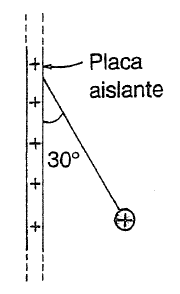
\includegraphics[scale=0.51]{figuras/fig_alvarenga_p862_17.png}
  \caption{Problema 24}
\end{figure}